\documentclass[11pt,a4paper]{article}
\usepackage[T1]{fontenc}
\usepackage[utf8]{inputenc}
\usepackage{lmodern}
\usepackage[margin=1in]{geometry}
\usepackage{amsmath,amssymb,amsthm,mathtools}
\usepackage{booktabs}
\usepackage{graphicx}
\usepackage{microtype}
\usepackage{xcolor}
\usepackage[colorlinks=true,linkcolor=blue!50!black,citecolor=blue!50!black,urlcolor=blue!50!black]{hyperref}

\newtheorem{theorem}{Theorem}
\newtheorem{proposition}[theorem]{Proposition}
\newtheorem{lemma}[theorem]{Lemma}
\newtheorem{corollary}[theorem]{Corollary}
\theoremstyle{definition}
\newtheorem{definition}[theorem]{Definition}
\theoremstyle{remark}
\newtheorem{remark}[theorem]{Remark}

\newcommand{\ket}[1]{\lvert #1\rangle}
\newcommand{\bra}[1]{\langle #1\rvert}
\newcommand{\ketbra}[2]{\lvert #1\rangle\langle #2\rvert}
\newcommand{\braket}[2]{\langle #1\vert #2\rangle}
\newcommand{\dA}{d_A}
\newcommand{\dB}{d_B}
\newcommand{\wA}{\omega_A}
\newcommand{\wB}{\omega_B}
\newcommand{\PiB}{\Pi_{\mathrm{Bell}}}
\newcommand{\cP}{\mathcal{P}}
\newcommand{\cC}{\mathcal{T}_{C}}
\newcommand{\cS}{\mathcal{T}_{S}}
\newcommand{\cE}{\mathcal{E}}
\newcommand{\Ad}{\operatorname{Ad}}
\newcommand{\tr}{\operatorname{Tr}}
\newcommand{\id}{\mathbf{1}}
\newcommand{\BD}{\mathrm{BD}}
\newcommand{\phib}[2]{\phi^{#1#2}}
% ---- Zenodo archive --------------------------------------------------------------------
% After the Zenodo DOI has been assigned, put it between the braces of \zenodoDOI, e.g.
%   \newcommand{\zenodoDOI}{10.5281/zenodo.1234567}
% The sentence in "Data and code availability" then appears automatically.
\newcommand{\zenodoDOI}{10.5281/zenodo.24432857}
\newcommand{\zenodonote}{\ifx\zenodoDOI\empty\else\ An archived snapshot of the repository
is available at Zenodo, \href{https://doi.org/\zenodoDOI}{doi:\zenodoDOI}.\fi}
% -----------------------------------------------------------------------------------------
\DeclareMathOperator{\lcm}{lcm}
\DeclareMathOperator{\spn}{span}

\hypersetup{pdftitle={Entanglement generation by unequal-dimension Bell-diagonal projections and a no-go theorem for local twirling},
  pdfauthor={Ruqing Chen}}

\title{Entanglement generation by unequal-dimension Bell-diagonal projections
and a no-go theorem for local twirling:\\
an audit and restoration of Phys.\ Rev.\ A 109, 012217 (2024)}
\author{Ruqing Chen\\[2pt]
\small Independent Researcher, Montreal, Quebec, Canada\\
\small \href{mailto:ruqing@hotmail.com}{ruqing@hotmail.com}\quad
ORCID: \href{https://orcid.org/0009-0009-4622-6615}{0009-0009-4622-6615}}
\date{November 17, 2026}

\begin{document}
\maketitle

\begin{abstract}
Moerland, Wyderka, Kampermann and Bru\ss{} recently introduced generalized Bell-diagonal
states on $\mathbb{C}^{\dA}\otimes\mathbb{C}^{\dB}$ with $\dA<\dB$ and stated, as their
Proposition~1, that a certain average over local unitaries equals the projection onto the
generalized Bell basis, so that this projection is a non-entangling channel. We show that
both parts of this statement fail whenever $\dA<\dB$. First, the local average is a
legitimate LOCC channel but it is not the Bell projection: it is not idempotent, it does not
fix the Bell states, its fixed-point algebra has dimension $\gcd(\dA,\dB)$, and its iterates
converge to a dephasing-and-shift twirl. Second, the Bell projection itself is entangling:
for every $2\le\dA<\dB$ we exhibit a pure product state whose projection has a partial
transpose with eigenvalue exactly $-1/(4\dA)$; in $2\times3$ this is a three-line computation
with rational numbers. We prove that the Bell projection is the unique positive
trace-preserving map that outputs Bell-diagonal states and fixes the Bell states, which
yields a no-go theorem: for $\dA<\dB$ no LOCC, separable, PPT or separability-preserving
channel can Bell-diagonalize, and any PPT-preserving channel stays at diamond distance at
least $1/(4\dA)$ from the projection. We identify the correct commuting pair of unitaries
that replaces the Heisenberg--Weyl pair, show that exactly one of them is nonlocal,
determine all local symmetries of the Bell basis, and check which results of the audited
paper are affected. The bound entangled states and the entanglement witnesses constructed
there do not rely on Proposition~1 and remain valid.
\end{abstract}

\section{Introduction}

Bell-diagonal states are a standard laboratory for bipartite entanglement theory. For two
$d$-level systems they are the mixtures of the $d^2$ maximally entangled states generated
from one of them by Heisenberg--Weyl operators; the resulting simplex has a rich geometry
and contains free, bound and separable states~\cite{BHN06,PH24,HHHH09}. A feature that
makes them especially useful is \emph{twirling}: averaging over the local unitaries
$X^\mu Z^\nu\otimes X^\mu Z^{-\nu}$ maps every state to its Bell-diagonal part. Since this
average is a mixture of local unitaries, it can be implemented by local operations and
classical communication (LOCC) and cannot create entanglement~\cite{BDSW96,Werner89}.
Entanglement found in the Bell-diagonal part of a state is therefore entanglement of the
state itself.

Moerland, Wyderka, Kampermann and Bru\ss{}~\cite{MWKB24} (MWKB in what follows) extended
Bell-diagonal states to unequal local dimensions $\dA<\dB$, constructed bound entangled
examples in dimensions $3\times4$ and $4\times6$, and generalized the family of separability
criteria of Sarbicki, Scala and Chru\'sci\'nski~\cite{SSC20} to non-Hermitian operator
bases. In Section~II of their paper they assert that the twirling property survives:
Proposition~1 of~\cite{MWKB24} states that an average $\Phi_1$ over $\dA\dB$ local unitaries
equals the projection $\PiB$ onto the generalized Bell basis, and concludes that this
projection is a non-entangling channel also if $\dA<\dB$.

The purpose of this paper is to show that this proposition is incorrect for every pair
$\dA<\dB$, to determine what is true instead, and to delimit the consequences. Throughout,
equation numbers of the form ``MWKB~(n)'' refer to the arXiv version
\texttt{2308.10607v2} of~\cite{MWKB24}, which was posted after acceptance and carries the
journal reference. Our results are the following.

\begin{enumerate}
\item \emph{Structure of the local average} (Theorem~\ref{thm:phi}). The map $\Phi_1$ of
MWKB~(19) factorizes as a block dephasing followed by an average over powers of the local
shift $X_A\otimes X_B$. It is an LOCC channel, but $\Phi_1=\PiB$ if and only if $\dA=\dB$.
For $\dA<\dB$ it maps the Bell state $\ket{\phib00}$ to a state of fidelity
$(\dA+1)(2\dA+1)/(6\dA^2)<1$ with it, the group generated by its Kraus unitaries has order
$\lcm(\dA,\dB)\,\dB\,(\dB/g)^{\dA}$ with $g=\gcd(\dA,\dB)$, its fixed points form a
$g$-dimensional algebra of diagonal operators, and $\Phi_1^{\,n}$ converges to the
corresponding twirl. For coprime dimensions the limit is the completely depolarizing
channel.
\item \emph{Entanglement generation} (Theorem~\ref{thm:neg}). For all $2\le\dA<\dB$ the
projection $\PiB$ maps an explicit pure product state to a state whose partial transpose
has the single negative eigenvalue $-1/(4\dA)$.
\item \emph{Uniqueness and no-go} (Proposition~\ref{prop:unique},
Theorem~\ref{thm:nogo}). The projection $\PiB$ is the only positive trace-preserving map
with Bell-diagonal outputs that fixes the Bell states. Hence, for $\dA<\dB$, no
separability-preserving or PPT-preserving channel, and in particular no LOCC channel,
performs Bell diagonalization.
\item \emph{What survives} (Lemma~\ref{lem:CD}, Proposition~\ref{prop:sym},
Section~\ref{sec:audit}). The Fourier representation of MWKB becomes correct once the local
shift is replaced by a block-cyclic shift $C$, which is nonlocal for $\dA<\dB$. The local
unitary symmetries of the Bell basis reduce to the dephasing group, whose twirl is the
block projection. The bound entangled states, the criteria and the witnesses of
Sections~III--V of~\cite{MWKB24} do not use Proposition~1 and are unaffected.
\end{enumerate}

All theorems, propositions and lemmas are established analytically. Numerical optimization
is used only for the lower bounds on the maximal entanglement generated from product
states that are reported in Table~\ref{tab:num}. In addition, every formula and every
number quoted below is reproduced by the deterministic script
\texttt{verify\_unequal\_bell\_projection.py} that accompanies this paper; it performs 116
checks, the decisive ones in exact rational arithmetic.

Our no-go result is related in spirit to the study of localizable operations by Beckman,
Gottesman, Nielsen and Preskill~\cite{BGNP01}, who showed that certain joint measurements
cannot be implemented by local operations. The setting here is different: we consider one
specific family of bases of maximally entangled states in unequal dimensions, classical
communication is allowed, and the obstruction is that the associated pinching map creates
entanglement with a non-positive partial transpose out of a product state.

\section{Setting and the commuting pair \texorpdfstring{$(C,D)$}{(C,D)}}

We use the conventions of~\cite{MWKB24}. Let $2\le\dA\le\dB$ and
$\mathcal{H}=\mathbb{C}^{\dA}\otimes\mathbb{C}^{\dB}$ with product basis $\ket{i,j}$,
$0\le i<\dA$, $0\le j<\dB$. For $S\in\{A,B\}$ let $X_S\ket{i}=\ket{i+1 \bmod d_S}$ and
$Z_S\ket{i}=\omega_S^{\,i}\ket{i}$ with $\omega_S=e^{2\pi \mathrm{i}/d_S}$. We write
$i\oplus\beta=(i+\beta)\bmod\dB$. The generalized Bell states are
\begin{equation}\label{eq:bell}
\ket{\phib\alpha\beta}=(Z_A^{\alpha}\otimes X_B^{\beta})\ket{\phib00}
=\frac{1}{\sqrt{\dA}}\sum_{i=0}^{\dA-1}\wA^{\alpha i}\ket{i,i\oplus\beta},
\qquad 0\le\alpha<\dA,\ 0\le\beta<\dB .
\end{equation}
They form an orthonormal basis of $\mathcal{H}$. We call a state Bell diagonal if it is
diagonal in this basis, denote the set of such states by $\BD$, and write
\begin{equation}\label{eq:Pi}
\PiB(\rho)=\sum_{\alpha,\beta}\bra{\phib\alpha\beta}\rho\ket{\phib\alpha\beta}\,
\ketbra{\phib\alpha\beta}{\phib\alpha\beta}
\end{equation}
for the orthogonal projection (pinching) onto $\BD$, which is the right-hand side of
MWKB~(20) at $q=1$.

The basis has a block structure. For $\beta\in\mathbb{Z}_{\dB}$ put
\begin{equation}\label{eq:V}
V_\beta=\spn\{\ket{i,i\oplus\beta}: 0\le i<\dA\},\qquad
\mathcal{H}=\bigoplus_{\beta=0}^{\dB-1}V_\beta ,
\end{equation}
and let $P_\beta$ be the projector onto $V_\beta$. The vector $\ket{i,j}$ lies in $V_\beta$
with $\beta=(j-i)\bmod\dB$, and the $\dA$ states $\ket{\phib\alpha\beta}$ with fixed
$\beta$ are the discrete Fourier basis of $V_\beta$.

MWKB introduce the modified clock operator $\tilde Z\ket{i}_A=\wB^{\,i}\ket{i}_A$ and the
local unitaries $T(\mu,\nu)=X_A^{\mu}\tilde Z^{\nu}\otimes X_B^{\mu}Z_B^{-\nu}$
(MWKB~(15),~(16)). We abbreviate
\begin{equation}\label{eq:SD}
S=T(1,0)=X_A\otimes X_B,\qquad D=T(0,1)=\tilde Z\otimes Z_B^{-1},\qquad
T(\mu,\nu)=S^{\mu}D^{\nu}.
\end{equation}
Since $D\ket{i,j}=\wB^{\,i-j}\ket{i,j}$, the operator $D$ acts on $V_\beta$ as the scalar
$\wB^{-\beta}$. The operator that plays the role of the shift is not $S$ but the
\emph{block-cyclic shift}
\begin{equation}\label{eq:C}
C\ket{i,j}=\begin{cases}\ket{i+1,\,j\oplus1}, & 0\le i<\dA-1,\\[2pt]
\ket{0,\,j\oplus(1-\dA)}, & i=\dA-1,\end{cases}
\end{equation}
which maps $\ket{i,i\oplus\beta}$ to $\ket{i',i'\oplus\beta}$ with $i'=(i+1)\bmod\dA$ and
thus permutes the basis of each $V_\beta$ cyclically. Figure~\ref{fig:shift} compares the
two shifts. Throughout, calligraphic letters denote maps on operators: $\cP$ is the
dephasing generated by $D$, and $\cC$ and $\cS$ are the averages over the powers of $C$
and of $S$.

\begin{figure}[t]
\centering
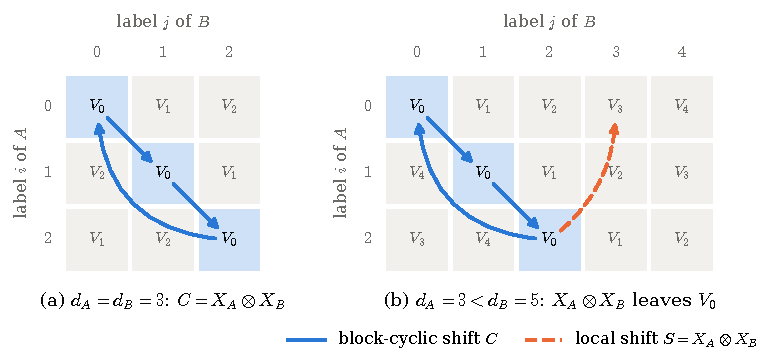
\includegraphics[width=0.92\textwidth]{fig_shift_mismatch.pdf}
\caption{The product basis $\ket{i,j}$ as a grid; each cell is labelled by the block
$V_\beta$, $\beta=(j-i)\bmod\dB$, that contains it, and $V_0$ is shaded. (a)~For
$\dA=\dB$ the local shift $X_A\otimes X_B$ moves along $V_0$ and closes up, so it
coincides with the block-cyclic shift $C$. (b)~For $\dA<\dB$ the label of $A$ wraps
around after $\dA$ steps but the label of $B$ does not: the local shift $S$ sends the
last vector of $V_0$ into $V_{\dA}$ (dashed), whereas $C$ returns it to $\ket{0,0}$. This
step of $C$ cannot be performed by a product of local operators.}
\label{fig:shift}
\end{figure}

\begin{lemma}\label{lem:CD}
Let $2\le\dA\le\dB$.
\begin{enumerate}
\item[(a)] $C$ and $D$ are commuting unitaries with $C^{\dA}=D^{\dB}=\id$, and
$C\ket{\phib\alpha\beta}=\wA^{-\alpha}\ket{\phib\alpha\beta}$,
$D\ket{\phib\alpha\beta}=\wB^{-\beta}\ket{\phib\alpha\beta}$.
\item[(b)] For every probability matrix $(p_{\alpha\beta})$ with Fourier coefficients
$\lambda_{\mu\nu}=\sum_{\alpha,\beta}p_{\alpha\beta}\wA^{\alpha\mu}\wB^{\beta\nu}$,
\begin{equation}\label{eq:fourier}
\sum_{\alpha,\beta}p_{\alpha\beta}\ketbra{\phib\alpha\beta}{\phib\alpha\beta}
=\frac{1}{\dA\dB}\sum_{\mu=0}^{\dA-1}\sum_{\nu=0}^{\dB-1}\lambda_{\mu\nu}\,C^{\mu}D^{\nu}.
\end{equation}
\item[(c)] $\PiB=\cC\circ\cP$ with the block dephasing and the block-cyclic average
\begin{equation}\label{eq:PC}
\cP(\rho)=\sum_{\beta}P_\beta\rho P_\beta=\frac{1}{\dB}\sum_{\nu=0}^{\dB-1}D^{\nu}\rho D^{-\nu},
\qquad
\cC(\rho)=\frac{1}{\dA}\sum_{\mu=0}^{\dA-1}C^{\mu}\rho\,C^{-\mu}.
\end{equation}
\item[(d)] $C=S$ if $\dA=\dB$. If $\dA<\dB$, then $C$ is not a product $U\otimes V$ of
local operators.
\end{enumerate}
\end{lemma}

\begin{proof}
(a) Both operators map each $V_\beta$ to itself; $D$ is scalar there and $C$ is the cyclic
shift of the $\dA$ basis vectors, whose eigenvectors are the Fourier vectors
\eqref{eq:bell} with eigenvalues $\wA^{-\alpha}$. (b) By (a) the joint spectral projector
of $(C,D)$ for the eigenvalue pair $(\wA^{-\alpha},\wB^{-\beta})$ is
$\ketbra{\phib\alpha\beta}{\phib\alpha\beta}
=(\dA\dB)^{-1}\sum_{\mu,\nu}\wA^{\alpha\mu}\wB^{\beta\nu}C^{\mu}D^{\nu}$; multiply by
$p_{\alpha\beta}$ and sum. (c) The average over the group
$\{C^{\mu}D^{\nu}\}\cong\mathbb{Z}_{\dA}\times\mathbb{Z}_{\dB}$ is the pinching onto its
joint eigenbasis, and it factorizes because $C$ and $D$ commute; the average over $D^\nu$
alone is the pinching onto the eigenspaces $V_\beta$ of $D$. (d) For $\dA=\dB$ the second
case of \eqref{eq:C} reads $\ket{0,j\oplus1}$, so $C=X_A\otimes X_B$. Let $\dA<\dB$ and
suppose $C=U\otimes V$. From $C\ket{0,j}=\ket{1,j\oplus1}$ we get
$V\ket{j}\propto\ket{j\oplus1}$, while $C\ket{\dA-1,j}=\ket{0,j\oplus(1-\dA)}$ gives
$V\ket{j}\propto\ket{j\oplus(1-\dA)}$. These agree only if $\dA\equiv0 \pmod{\dB}$, which
is excluded by $0<\dA<\dB$.
\end{proof}

Equation~\eqref{eq:fourier} is the correct form of MWKB~(17). For $\dA=\dB$ it reduces to
the familiar representation MWKB~(18), because then $C=X\otimes X$ and $D=Z\otimes Z^{-1}$.
For $\dA<\dB$ the right-hand side of MWKB~(17), which has $T(\mu,\nu)=S^\mu D^\nu$ in place
of $C^\mu D^\nu$, is in general not even Hermitian: for $p_{\alpha\beta}=\delta_{\alpha0}\delta_{\beta0}$
it equals $\dA^{-1}\sum_{\mu<\dA}S^{\mu}P_0$, whose $\mu=1$ term contains
$\ketbra{0,\dA}{\dA-1,\dA-1}$ without its adjoint.

\section{The true structure of the local average \texorpdfstring{$\Phi_1$}{Phi1}}

MWKB~(19) defines, for $q\in[0,1]$,
\begin{equation}\label{eq:Phi}
\Phi_q(\rho)=(1-q)\rho+\frac{q}{\dA\dB}\sum_{\mu=0}^{\dA-1}\sum_{\nu=0}^{\dB-1}
T(\mu,\nu)\,\rho\,T(\mu,\nu)^{\dagger},
\end{equation}
and Proposition~1 of~\cite{MWKB24} asserts
$\Phi_q(\rho)=(1-q)\rho+q\,\PiB(\rho)$ for all $\rho$ (MWKB~(20)). The proof offered there
rests on the identity $\tilde Z^{\nu}X_A^{\mu}=\wB^{\mu\nu}X_A^{\mu}\tilde Z^{\nu}$
(MWKB~(21)). This identity does not hold for $\dA<\dB$: one finds
$\tilde Z X_A\ket{i}=\wB\,X_A\tilde Z\ket{i}$ for $i<\dA-1$, but
$\tilde Z X_A\ket{\dA-1}=\ket{0}$ whereas
$\wB\,X_A\tilde Z\ket{\dA-1}=\wB^{\,\dA}\ket{0}$, that is,
\begin{equation}\label{eq:mismatch}
\tilde Z X_A=\wB\,X_A\tilde Z\,\bigl(\id+(\wB^{-\dA}-1)\ketbra{\dA-1}{\dA-1}\bigr),
\end{equation}
because $X_A$ wraps around modulo $\dA$ whereas the phases of $\tilde Z$ are defined
modulo $\dB$. The mismatch factor $\eta^{-1}$, with
\begin{equation}\label{eq:eta}
\eta=\wB^{\,\dA},\qquad \eta\neq1 \text{ for } \dA<\dB,\qquad
\operatorname{ord}(\eta)=\dB/g,\quad g=\gcd(\dA,\dB),
\end{equation}
governs everything that follows.

\begin{theorem}\label{thm:phi}
Let $2\le\dA\le\dB$, $g=\gcd(\dA,\dB)$, and let $G$ be the group generated by the unitaries
$T(\mu,\nu)$.
\begin{enumerate}
\item[(i)] $\Phi_1=\cS\circ\cP$, where $\cP$ is the block dephasing \eqref{eq:PC} and
$\cS(\rho)=\dA^{-1}\sum_{\mu=0}^{\dA-1}S^{\mu}\rho S^{-\mu}$. Every $\Phi_q$ is a mixture
of local unitaries, hence an LOCC channel.
\item[(ii)] If $\dA<\dB$, then
\begin{equation}\label{eq:fid}
\bra{\phib00}\Phi_1\bigl(\ketbra{\phib00}{\phib00}\bigr)\ket{\phib00}
=\frac{(\dA+1)(2\dA+1)}{6\dA^{2}}<1 .
\end{equation}
Consequently $\Phi_1=\PiB$ if and only if $\dA=\dB$, and for $\dA<\dB$ the channel
$\Phi_1$ neither fixes the Bell states nor is idempotent.
\item[(iii)] $G$ is a semidirect product of the diagonal group
$\Delta=\langle D\rangle\times\{\operatorname{diag}(\eta^{k_0},\dots,\eta^{k_{\dA-1}})\otimes\id\}$
by the cyclic group $\langle S\rangle$, and
\begin{equation}\label{eq:order}
|G|=\lcm(\dA,\dB)\cdot\dB\cdot\Bigl(\frac{\dB}{g}\Bigr)^{\dA}.
\end{equation}
\item[(iv)] If $\dA<\dB$, the fixed-point set of $\Phi_1$ is the commutant of $G$, namely
$\spn\{Q_r: r\in\mathbb{Z}_g\}$ with
$Q_r=\sum_{(j-i)\equiv r\ (\mathrm{mod}\ g)}\ketbra{i,j}{i,j}$, and
\begin{equation}\label{eq:limit}
\lim_{n\to\infty}\Phi_1^{\,n}(\rho)=\cE(\rho):=\sum_{r\in\mathbb{Z}_g}
\frac{\tr(Q_r\rho)}{\tr Q_r}\,Q_r,\qquad \tr Q_r=\frac{\dA\dB}{g}.
\end{equation}
In particular, for coprime $\dA<\dB$ the iterates of $\Phi_1$ converge to the completely
depolarizing channel.
\end{enumerate}
\end{theorem}

\begin{proof}
(i) By \eqref{eq:SD}, the sum over $\nu$ in \eqref{eq:Phi} is the average over the powers
of $D$, which is $\cP$ by Lemma~\ref{lem:CD}(c), and the remaining sum over $\mu$ is
$\cS$.

(ii) Since $\ket{\phib00}\in V_0$, $\cP$ leaves its projector unchanged, and the left-hand
side of \eqref{eq:fid} equals $\dA^{-1}\sum_{\mu<\dA}|\bra{\phib00}S^{\mu}\ket{\phib00}|^{2}$.
Now $S^{\mu}\ket{i,i}=\ket{(i+\mu)\bmod\dA,\,(i+\mu)\bmod\dB}$. For $0\le\mu<\dA$ this vector
is again of the form $\ket{k,k}$ if $i+\mu<\dA$; if $i+\mu\ge\dA$ its first label is
$i+\mu-\dA$ and its second label is $i+\mu$ or $i+\mu-\dB$, and these coincide only when
$\dA=\dB$. Hence $\bra{\phib00}S^{\mu}\ket{\phib00}=(\dA-\mu)/\dA$ for $\dA<\dB$, and
$\dA^{-3}\sum_{m=1}^{\dA}m^{2}$ gives \eqref{eq:fid}. The value is below $1$ for
$\dA\ge2$, whereas $\PiB$ fixes $\ketbra{\phib00}{\phib00}$. If $\Phi_1$ were idempotent it
would fix its own outputs; by part (iv), proved below, its fixed points are diagonal in
the product basis, while $\Phi_1(\ketbra{\phib00}{\phib00})$ has the nonzero off-diagonal
entry $\dA^{-2}$ between $\ket{0,0}$ and $\ket{1,1}$ and so is not diagonal.
For $\dA=\dB$ we have $S=C$ by Lemma~\ref{lem:CD}(d), so $\Phi_1=\cC\circ\cP=\PiB$.

(iii) $G$ is generated by $S$ and $D$. A direct computation gives, for $1\le k\le\dA$,
\begin{equation}\label{eq:Fk}
D^{-1}S^{-k}DS^{k}=F_k\otimes\id,\qquad
F_k=\operatorname{diag}\bigl(\eta^{-[\,i\ge\dA-k\,]}\bigr)_{i=0}^{\dA-1},
\end{equation}
where $[\cdot]$ is $1$ if the condition holds and $0$ otherwise. The quotients
$F_kF_{k-1}^{-1}$ (with $F_0=\id$) are the operators $E_i^{-1}$, where $E_i$ multiplies
$\ket{i}_A$ by $\eta$ and fixes the other basis vectors, for $i=\dA-k$. Hence $G$ contains
$E_0,\dots,E_{\dA-1}$, and $\Delta=\langle D,E_0,\dots,E_{\dA-1}\rangle$ is abelian of order
$\dB(\dB/g)^{\dA}$: the $E_i$ generate $(\mathbb{Z}_{\dB/g})^{\dA}$, and a power $D^{a}$
is independent of the label $j$ only if $\dB\mid a$. Conjugation by $S$ permutes the
$E_i$ cyclically, and $S^{-1}DS=D(F_1\otimes\id)$ by \eqref{eq:Fk}, so $\Delta$ is normal
in $G$. Finally $S^{m}\in\Delta$ only if $S^{m}$ is diagonal, i.e.\ only if
$\lcm(\dA,\dB)$ divides $m$, in which case $S^m=\id$. This gives \eqref{eq:order}.

(iv) Let $\Phi_1(\rho)=\rho$. Then
\begin{equation*}
\|\rho\|_2=\Bigl\|\frac{1}{\dA\dB}\sum_{\mu,\nu}T(\mu,\nu)\,\rho\,T(\mu,\nu)^{\dagger}\Bigr\|_2 ,
\end{equation*}
where every term of the average has Hilbert--Schmidt norm $\|\rho\|_2$. This norm is
strictly convex, so all terms $T(\mu,\nu)\rho T(\mu,\nu)^{\dagger}$ must coincide; as
$T(0,0)=\id$, they equal $\rho$.
Thus $\rho$ commutes with $S$ and $D$, hence with $G$; the converse is obvious. An operator
commuting with every $E_i$ is block diagonal with respect to the label $i$ (here
$\eta\neq1$ is used), and one commuting with $D$ is block diagonal with respect to
$(j-i)\bmod\dB$; together, it is diagonal in the product basis. Commuting with $S$ then
means being constant on the orbits of $(i,j)\mapsto(i+1,j+1)$ on
$\mathbb{Z}_{\dA}\times\mathbb{Z}_{\dB}$, which are the $g$ classes $(j-i)\bmod g$. For the
limit, the same norm argument applied to $\Phi_1(X)=\lambda X$ with $|\lambda|=1$ shows
$\lambda=1$, so $1$ is the only eigenvalue of modulus one of the contraction $\Phi_1$, and
$\Phi_1^{\,n}$ converges to a projection onto the fixed-point space. The map $\cE$ is the
orthogonal projection onto that space and satisfies $\cE\Phi_1=\Phi_1\cE=\cE$, so it is the
limit.
\end{proof}

Two examples illustrate part (iv). For $2\times3$ the dimensions are coprime, $|G|=162$,
the only fixed points are the multiples of the identity, and
$\Phi_1^{\,n}(\rho)\to\id/6$ for every state; the second-largest eigenvalue modulus of
$\Phi_1$ is $\sqrt3/2$, which sets the rate of convergence. For $2\times4$ one has $g=2$
and $|G|=64$, the fixed points are spanned by the two projectors $Q_0$ and $Q_1$ onto the
product vectors $\ket{i,j}$ with $j-i$ even and odd, respectively, and the limit retains
only the single classical parameter $\tr(Q_0\rho)$.

Theorem~\ref{thm:phi} shows that the two halves of Proposition~1 of~\cite{MWKB24} belong to
two different maps. The map defined by MWKB~(19) is non-entangling, but it does not
produce Bell-diagonal states. The map on the right-hand side of MWKB~(20) produces
Bell-diagonal states, but, as we show next, it is entangling.

\section{Entanglement generation by the Bell projection}

\subsection{The \texorpdfstring{$2\times3$}{2x3} example}

Take $\dA=2$, $\dB=3$ and the product state
$\ket{\psi}=\tfrac12(\ket0+\ket1)\otimes(\ket0+\ket1)$. The Bell basis is
$\ket{\phib{\alpha}{\beta}}=(\ket{0,\beta}+(-1)^{\alpha}\ket{1,\beta\oplus1})/\sqrt2$, and the
populations $p_{\alpha\beta}=|\braket{\phib\alpha\beta}{\psi}|^{2}$ are
\begin{equation}\label{eq:pop23}
p_{00}=\tfrac12,\qquad p_{10}=0,\qquad p_{01}=p_{11}=p_{02}=p_{12}=\tfrac18 .
\end{equation}
Equal weights on $\ket{\phib0\beta}$ and $\ket{\phib1\beta}$ add up to an incoherent
mixture, so
\begin{equation}\label{eq:sigma23}
\PiB(\ketbra\psi\psi)=\tfrac12\ketbra{\phib00}{\phib00}
+\tfrac18\bigl(\ketbra{01}{01}+\ketbra{12}{12}+\ketbra{02}{02}+\ketbra{10}{10}\bigr).
\end{equation}
Partial transposition on $A$ moves the coherence $\tfrac14\ketbra{00}{11}$ of the first
term to $\tfrac14\ketbra{10}{01}$. On $\spn\{\ket{01},\ket{10}\}$ the partial transpose is
therefore
\begin{equation}\label{eq:block23}
\begin{pmatrix}\tfrac18&\tfrac14\\[2pt]\tfrac14&\tfrac18\end{pmatrix},
\qquad\text{with eigenvalues } \tfrac38 \text{ and } -\tfrac18 .
\end{equation}
A product state is mapped to a state with a non-positive partial
transpose~\cite{Peres96,HHH96}. The full spectrum of the partial transpose is
$\{-\tfrac18,\tfrac18,\tfrac18,\tfrac14,\tfrac14,\tfrac38\}$.

\subsection{All dimensions \texorpdfstring{$2\le d_A<d_B$}{2 <= dA < dB}}

\begin{theorem}\label{thm:neg}
Let $2\le\dA<\dB$ and
$\rho_\star=\ketbra{a}{a}\otimes\ketbra{b}{b}$ with
$\ket{a}=(\ket0+\ket1)/\sqrt2\in\mathbb{C}^{\dA}$ and
$\ket{b}=(\ket0+\ket1)/\sqrt2\in\mathbb{C}^{\dB}$. Then the partial transpose of
$\PiB(\rho_\star)$ has exactly one negative eigenvalue,
\begin{equation}\label{eq:lmin}
\lambda_{\min}\bigl(\PiB(\rho_\star)^{T_A}\bigr)=-\frac{1}{4\dA},\qquad
\text{with eigenvector } \ket{v}=\frac{\ket{\dA-1,0}-\ket{0,\dA-1}}{\sqrt2},
\end{equation}
so the negativity~\cite{VW02} of $\PiB(\rho_\star)$ equals $1/(4\dA)$. Moreover
$\bra{v}\bigl[(1-q)\rho_\star+q\,\PiB(\rho_\star)\bigr]^{T_A}\ket{v}=-q/(4\dA)$, so the
right-hand side of MWKB~(20) is an entangling map for every $q\in(0,1]$.
\end{theorem}

\begin{proof}
We use $\PiB=\cC\circ\cP$. The four product vectors in $\rho_\star$ lie in
$V_0$ ($\ket{0,0}$, $\ket{1,1}$), $V_1$ ($\ket{0,1}$) and $V_{\dB-1}$ ($\ket{1,0}$), and
these blocks are distinct because $\dB\ge3$. Hence
\begin{equation*}
\cP(\rho_\star)=\tfrac14(\ket{0,0}+\ket{1,1})(\bra{0,0}+\bra{1,1})
+\tfrac14\ketbra{0,1}{0,1}+\tfrac14\ketbra{1,0}{1,0}.
\end{equation*}
The average $\cC$ replaces each operator $\ketbra{i,i\oplus\beta}{i',i'\oplus\beta}$ by the
mean of its $\dA$ cyclic translates inside $V_\beta$. Writing $\ket{k,k}$ for
$\ket{k}_A\ket{k}_B$ with $0\le k<\dA$ and $k^{+}=(k+1)\bmod\dA$,
\begin{equation}\label{eq:sigma}
\PiB(\rho_\star)=\frac{1}{4\dA}\Bigl[\,2P_0+P_1+P_{\dB-1}
+\sum_{k=0}^{\dA-1}\bigl(\ketbra{k^{+},k^{+}}{k,k}+\ketbra{k,k}{k^{+},k^{+}}\bigr)\Bigr].
\end{equation}
The projectors are diagonal and invariant under partial transposition, while
$\ketbra{k^{+},k^{+}}{k,k}^{T_A}=\ketbra{k,k^{+}}{k^{+},k}$. Therefore
\begin{equation}\label{eq:sigmaPT}
\PiB(\rho_\star)^{T_A}=\frac{1}{4\dA}\Bigl[\,2P_0+P_1+P_{\dB-1}
+\sum_{k=0}^{\dA-1}\bigl(\ketbra{k,k^{+}}{k^{+},k}+\ketbra{k^{+},k}{k,k^{+}}\bigr)\Bigr].
\end{equation}
For $0\le k\le\dA-2$ the vectors $\ket{k,k+1}$ and $\ket{k+1,k}$ belong to $V_1$ and
$V_{\dB-1}$ and carry the diagonal weight $1/(4\dA)$. The wrap-around term $k=\dA-1$
couples $\ket{\dA-1,0}\in V_{\dB-\dA+1}$ with $\ket{0,\dA-1}\in V_{\dA-1}$.

\emph{Case $\dA\ge3$.} Then $2\le\dA-1\le\dB-2$ and $2\le\dB-\dA+1\le\dB-2$, so the two
wrap-around vectors lie outside $V_0\oplus V_1\oplus V_{\dB-1}$ and have zero diagonal
weight. The operator \eqref{eq:sigmaPT} is a direct sum of the block
$(4\dA)^{-1}\bigl(\begin{smallmatrix}0&1\\1&0\end{smallmatrix}\bigr)$ on
$\spn\{\ket{\dA-1,0},\ket{0,\dA-1}\}$, of $\dA-1$ positive semidefinite blocks
$(4\dA)^{-1}\bigl(\begin{smallmatrix}1&1\\1&1\end{smallmatrix}\bigr)$, and of a
non-negative diagonal remainder. The only negative eigenvalue is $-1/(4\dA)$.

\emph{Case $\dA=2$.} The terms $k=0$ and $k=1$ both couple $\ket{0,1}\in V_1$ with
$\ket{1,0}\in V_{\dB-1}$, which gives the block
$\tfrac18\bigl(\begin{smallmatrix}1&2\\2&1\end{smallmatrix}\bigr)$ with eigenvalues
$\tfrac38$ and $-\tfrac18=-1/(4\dA)$; everything else is diagonal and non-negative.

Finally, $\rho_\star^{T_A}=\rho_\star$ because $\ket a$ is real, and
$\braket{v}{a,b}=(a_{\dA-1}b_0-a_0b_{\dA-1})/\sqrt2=0$ in both cases, which gives the
statement about $(1-q)\rho_\star+q\PiB(\rho_\star)$.
\end{proof}

Theorem~\ref{thm:neg} holds for every pair $2\le\dA<\dB$, whether or not the dimensions
are coprime and whether or not $\dA$ divides $\dB$: the Bell projection is entangling on
the whole class of unequal-dimensional systems.

\subsection{Why equal dimensions are protected}

The mechanism is shown in Fig.~\ref{fig:mech}. Cyclic symmetrization inside $V_0$ creates
the wrap-around coherence between $\ket{\dA-1,\dA-1}$ and $\ket{0,0}$. Partial
transposition moves every coherence of $V_0$ to a pair of off-diagonal cells
$\ket{k,k^{+}}$, $\ket{k^{+},k}$, and such a pair is harmless only if both cells carry
enough diagonal weight. The pairs with $k\le\dA-2$ always lie in $V_1$ and $V_{\dB-1}$,
which the input populates. For the wrap-around pair $\ket{\dA-1,0}$, $\ket{0,\dA-1}$ this
is true if and only if $\dA=\dB$: then the two cells again belong to $V_1$ and $V_{\dB-1}$,
the corresponding block of the partial transpose is
$(4\dA)^{-1}\bigl(\begin{smallmatrix}1&1\\1&1\end{smallmatrix}\bigr)\ge0$, and the output
is PPT, as it must be for an LOCC twirl. For $\dA<\dB$ the two cells belong to
$V_{\dB-\dA+1}$ and $V_{\dA-1}$, which the input does not populate, and the coherence is
left uncompensated. In short, the block structure is periodic with period $\dB$ while the
symmetrization is periodic with period $\dA$, and the two periodicities are compatible at
the boundary only when they are equal.

\begin{figure}[t]
\centering
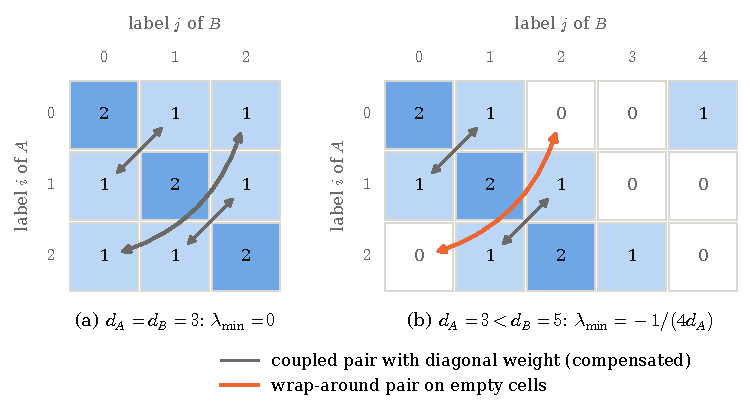
\includegraphics[width=0.92\textwidth]{fig_mechanism.pdf}
\caption{Diagonal weights of $\PiB(\rho_\star)$ in units of $1/(4\dA)$ on the product
basis, and the pairs of cells coupled by the off-diagonal entries of its partial
transpose, each of strength $1/(4\dA)$. (a)~$\dA=\dB=3$: every coupled pair sits on
populated cells and the partial transpose is positive semidefinite. (b)~$\dA=3$,
$\dB=5$: the wrap-around pair $\ket{2,0}$, $\ket{0,2}$ sits on empty cells, which
produces the eigenvalue $-1/(4\dA)$ of Theorem~\ref{thm:neg}.}
\label{fig:mech}
\end{figure}

\subsection{Numerical lower bounds on the maximal entanglement}

The state $\rho_\star$ is in general not the product state for which $\PiB$ generates the
most entanglement. Table~\ref{tab:num} and Fig.~\ref{fig:neg} give, for the eight smallest
dimension pairs, the largest negativity of $\PiB(\ketbra{a}{a}\otimes\ketbra{b}{b})$ found
by numerical optimization over product states. The vectors $a$ and $b$ are parametrized
by the real and imaginary parts of their components and normalized inside the objective
function. Each run consists of a quasi-Newton (BFGS) search followed by a Nelder--Mead
refinement; we use between 20 and 60 random starting points per dimension pair, drawn
from a seeded generator, together with two structured starting points, and every optimum
is re-evaluated through an independent implementation of $\PiB$. The reported values are
the best local optima found. They are rigorous lower bounds on the maximum but not
certified global maxima. For $3\times4$ and $3\times6$ they agree to six digits with
$\sqrt2/6$, and for $4\times6$ with $3/8$; we have not attempted to prove optimality.

\begin{figure}[t]
\centering
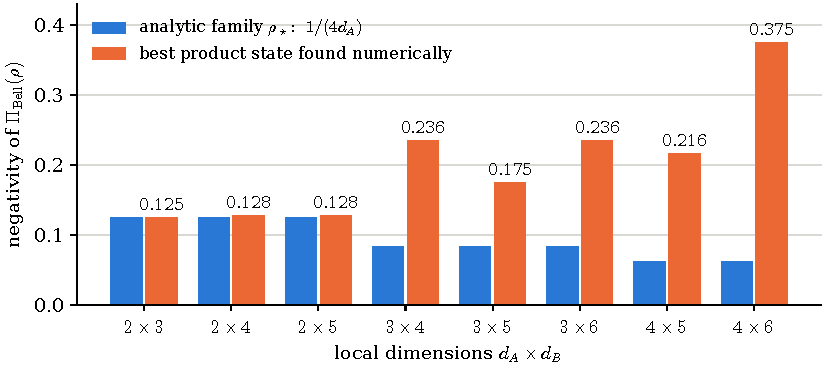
\includegraphics[width=0.86\textwidth]{fig_negativity.pdf}
\caption{Negativity generated by the Bell projection from product states: the analytic
value $1/(4\dA)$ for $\rho_\star$ (Theorem~\ref{thm:neg}) and the best value found by
numerical optimization over all product states (lower bounds, see
Table~\ref{tab:num}).}
\label{fig:neg}
\end{figure}

\begin{table}[t]
\centering
\caption{Data for $\dA<\dB$. $|G|$ is the order \eqref{eq:order}, confirmed by exhaustive
enumeration; $F$ is the fidelity \eqref{eq:fid}; $\dim\mathrm{Fix}$ is the dimension of the
fixed-point space of $\Phi_1$; the last two columns give the negativity of
$\PiB(\rho_\star)$ from Theorem~\ref{thm:neg} and the largest negativity of
$\PiB$ applied to a product state found numerically (a lower bound on the maximum).}
\label{tab:num}
\begin{tabular}{cccccc}
\toprule
$\dA\times\dB$ & $|G|$ & $F$ & $\dim\mathrm{Fix}(\Phi_1)$ & $1/(4\dA)$ & numerical max.\\
\midrule
$2\times3$ & $162$ & $5/8$ & $1$ & $0.1250$ & $0.1250$\\
$2\times4$ & $64$ & $5/8$ & $2$ & $0.1250$ & $0.1280$\\
$2\times5$ & $1250$ & $5/8$ & $1$ & $0.1250$ & $0.1280$\\
$3\times4$ & $3072$ & $14/27$ & $1$ & $0.0833$ & $0.2357$\\
$3\times5$ & $9375$ & $14/27$ & $1$ & $0.0833$ & $0.1754$\\
$3\times6$ & $288$ & $14/27$ & $3$ & $0.0833$ & $0.2357$\\
$4\times5$ & $62500$ & $15/32$ & $1$ & $0.0625$ & $0.2164$\\
$4\times6$ & $5832$ & $15/32$ & $2$ & $0.0625$ & $0.3750$\\
\bottomrule
\end{tabular}
\end{table}

\section{A no-go theorem for Bell diagonalization}

One might hope that some other channel achieves what $\Phi_1$ does not: Bell-diagonal
outputs without touching states that are already Bell diagonal. The following proposition
shows that there is no freedom.

\begin{definition}\label{def:bd}
A linear map $\Lambda$ on operators of $\mathcal{H}$ is \emph{Bell diagonalizing} if it is
positive and trace preserving, $\Lambda(\rho)\in\BD$ for all states $\rho$, and
$\Lambda(\ketbra{\phib\alpha\beta}{\phib\alpha\beta})=\ketbra{\phib\alpha\beta}{\phib\alpha\beta}$
for all $\alpha,\beta$.
\end{definition}

\begin{proposition}\label{prop:unique}
Let $\{\ket{e_k}\}$ be an orthonormal basis of a finite-dimensional Hilbert space, with
projectors $\phi_k=\ketbra{e_k}{e_k}$, and let $\Lambda$ be a positive trace-preserving
linear map such that $\Lambda(\rho)$ is diagonal in this basis for every $\rho$ and
$\Lambda(\phi_k)=\phi_k$ for every $k$. Then $\Lambda$ is the pinching
$\rho\mapsto\sum_k\phi_k\rho\,\phi_k$. In particular, for all $\dA\le\dB$ the projection
$\PiB$ is the unique Bell-diagonalizing map.
\end{proposition}

\begin{proof}
Since the outputs are diagonal in the basis,
$\Lambda(\rho)=\sum_k\tr(A_k\rho)\,\phi_k$ with $A_k=\Lambda^{\dagger}(\phi_k)$. The adjoint of a positive trace-preserving map is positive
and unital, so $A_k\ge0$ and $\sum_kA_k=\id$, whence $0\le A_k\le\id$. The fixed-point
condition gives $\tr(A_k\phi_l)=\delta_{kl}$. From $\bra{e_k}(\id-A_k)\ket{e_k}=0$
and $\id-A_k\ge0$ we get $A_k\ket{e_k}=\ket{e_k}$, and from
$\bra{e_l}A_k\ket{e_l}=0$ and $A_k\ge0$ we get $A_k\ket{e_l}=0$ for $l\neq k$.
Hence $A_k=\phi_k$, and $\Lambda$ is the pinching. For the Bell basis the pinching is
$\PiB$.
\end{proof}

We use the following terminology. A channel is \emph{PPT preserving} if it maps every
state with positive partial transpose to a state with positive partial transpose, and
\emph{separability preserving}, or non-entangling~\cite{BP08}, if it maps separable
states to separable states. A \emph{PPT operation} in the sense of Rains~\cite{Rains01}
is a channel $\Lambda$ for which $T_A\circ\Lambda\circ T_A$ is completely positive; every
PPT operation is PPT preserving, but the converse does not hold. Our counterexample
excludes the larger class, and in fact any channel that maps product states to PPT
states.

Recall the standard hierarchy: mixtures of local unitaries are LOCC, LOCC channels are
separable, and separable channels are PPT operations~\cite{Rains01,CLMOW14}. Separable
channels are separability preserving, and all channels in the hierarchy are PPT
preserving.

\begin{theorem}[No-go]\label{thm:nogo}
Let $2\le\dA<\dB$.
\begin{enumerate}
\item[(a)] No Bell-diagonalizing map preserves separability or positivity of the partial
transpose. In particular, there is no LOCC channel, no separable channel, no PPT
operation and no mixture of local unitaries that maps every state to a Bell-diagonal
state while fixing the Bell states.
\item[(b)] Every channel $\Lambda$ that maps product states to PPT states satisfies
\begin{equation}\label{eq:diamond}
\bigl\|\Lambda(\rho_\star)-\PiB(\rho_\star)\bigr\|_1\ \ge\ \frac{1}{4\dA},
\end{equation}
with $\rho_\star$ from Theorem~\ref{thm:neg}; hence
$\|\Lambda-\PiB\|_\diamond\ge 1/(4\dA)$.
\end{enumerate}
In contrast, for $\dA=\dB$ the projection $\PiB$ is a mixture of the local unitaries
$X^{\mu}Z^{\nu}\otimes X^{\mu}Z^{-\nu}$.
\end{theorem}

\begin{proof}
(a) By Proposition~\ref{prop:unique} such a map equals $\PiB$, and by
Theorem~\ref{thm:neg} it sends the product state $\rho_\star$ to a state that is not PPT,
hence not separable. (b) Let $\tau=\Lambda(\rho_\star)$ and $\sigma=\PiB(\rho_\star)$. With
$\ket v$ from \eqref{eq:lmin}, $\bra v\tau^{T_A}\ket v\ge0$ and
$\bra v\sigma^{T_A}\ket v=-1/(4\dA)$, so
$1/(4\dA)\le\bra v(\tau-\sigma)^{T_A}\ket v\le\|(\tau-\sigma)^{T_A}\|_2=\|\tau-\sigma\|_2
\le\|\tau-\sigma\|_1$, where we used that partial transposition preserves the
Hilbert--Schmidt norm. The last statement is Lemma~\ref{lem:CD}(c),(d).
\end{proof}

The bound \eqref{eq:diamond} is a universal lower bound obtained from the single input
$\rho_\star$; we do not claim that it is tight, and the larger negativities in
Table~\ref{tab:num} indicate that it is not.

What can be done locally is determined by the local symmetries of the Bell basis.

\begin{proposition}\label{prop:sym}
Let $2\le\dA<\dB$. A product unitary $U\otimes V$ commutes with all Bell projectors
$\ketbra{\phib\alpha\beta}{\phib\alpha\beta}$ if and only if
$U\otimes V=e^{\mathrm{i}\gamma}D^{\nu}$ for some $\gamma\in\mathbb{R}$ and
$\nu\in\mathbb{Z}_{\dB}$. The twirl over this group is the block dephasing $\cP$.
\end{proposition}

\begin{proof}
Powers of $D$ commute with the Bell projectors by Lemma~\ref{lem:CD}(a). Conversely, let
$U\otimes V$ commute with all of them. Then it commutes with each
$P_\beta=\sum_\alpha\ketbra{\phib\alpha\beta}{\phib\alpha\beta}$ and maps $V_\beta$ to
itself. A vector $\sum_ic_i\ket{i,i\oplus\beta}$ of $V_\beta$ has Schmidt rank equal to the
number of nonzero $c_i$, so the product vector $U\ket i\otimes V\ket{i\oplus\beta}$ must be
proportional to a single $\ket{k,k\oplus\beta}$. Thus $U\ket i\propto\ket{\pi(i)}$ for a
permutation $\pi$ of $\{0,\dots,\dA-1\}$, and
$V\ket{i\oplus\beta}\propto\ket{\pi(i)\oplus\beta}$ for all $i$ and $\beta$. Taking
$j=i\oplus\beta$ shows that $V\ket j\propto\ket{j\oplus(\pi(i)-i)}$ for every $i$, so
$\pi(i)\equiv i+t \pmod{\dB}$ with $t=\pi(0)\in\{0,\dots,\dA-1\}$. If $t\ge1$, the choice
$i=\dA-t$ gives $\pi(i)\equiv\dA\pmod{\dB}$, which is impossible for
$0\le\pi(i)<\dA<\dB$. Hence $t=0$ and $U=\operatorname{diag}(u_i)$,
$V=\operatorname{diag}(v_j)$ are diagonal. The Bell states are eigenvectors of such a
product if and only if $u_iv_{i\oplus\beta}=c_\beta$ does not depend on $i$. Then
$v_\beta=c_\beta/u_0$ and $c_{\beta\oplus i}=c_\beta\,u_0/u_i$; with $r=u_0/u_1$ this gives
$c_\beta=c_0r^{\beta}$, $r^{\dB}=1$, $u_i=u_0r^{-i}$ and $v_j=(c_0/u_0)\,r^{j}$, i.e.\
$U\otimes V=c_0\operatorname{diag}(r^{\,j-i})=c_0D^{-\nu}$ for $r=\wB^{\nu}$. The twirl is
$\cP$ by \eqref{eq:PC}.
\end{proof}

For $\dA=\dB$ the same argument allows every $t$, and the symmetry group additionally
contains the powers of $S=C$. Proposition~\ref{prop:sym} thus pinpoints what is lost in
unequal dimensions: the shift symmetry ceases to be local. We collect the positive
statements.

\begin{corollary}\label{cor:restore}
Let $2\le\dA<\dB$.
\begin{enumerate}
\item[(a)] The block dephasing $\cP$ is a mixture of local unitaries, fixes every
Bell-diagonal state, and maps every state to a state that is block diagonal with respect
to $\bigoplus_\beta V_\beta$. If $\cP(\rho)$ is entangled, then $\rho$ is entangled.
\item[(b)] $\PiB=\cC\circ\cP$, and a block-diagonal state is Bell diagonal if and only if
it commutes with the nonlocal unitary $C$.
\item[(c)] The inference ``$\PiB(\rho)$ entangled $\Rightarrow$ $\rho$ entangled'' is
invalid; $\rho_\star$ is a counterexample. The inference
``$\Phi_1(\rho)$ entangled $\Rightarrow$ $\rho$ entangled'' is valid, but $\Phi_1(\rho)$ is
in general not Bell diagonal.
\end{enumerate}
\end{corollary}

\begin{remark}\label{rem:divisible}
Theorem~\ref{thm:nogo} is a statement about the specific basis \eqref{eq:bell}, in which
the shift on $B$ runs modulo $\dB$; it is not a statement about all orthonormal bases of
maximally entangled states in unequal dimensions. If $\dA$ divides $\dB$, write $\mathbb{C}^{\dB}=\mathbb{C}^{\dA}\otimes\mathbb{C}^{m}$
with $m=\dB/\dA$ and consider instead the orthonormal basis
$\ket{\phi^{\alpha\beta}_{\dA}}\otimes\ket{k}$ built from the ordinary $\dA\times\dA$ Bell
states and $0\le k<m$. Its vectors are again maximally entangled of Schmidt rank $\dA$, and
the projection onto it is the twirl over the local unitaries
$X\otimes(X\otimes\id)$, $Z\otimes(Z^{-1}\otimes\id)$ and $\id\otimes(\id\otimes Z_m)$,
hence LOCC. Whether a basis of maximally entangled states of Schmidt rank $\dA$ with a
non-entangling projection exists when $\dA$ does not divide $\dB$, for instance in
$2\times3$, is a question we leave open.
\end{remark}

\section{Audit of the downstream results of the audited paper}\label{sec:audit}

We now go through~\cite{MWKB24} and record which statements depend on Proposition~1 or on
the identities shown above to fail. All numerical statements in this section were
recomputed by the accompanying script from the definitions \eqref{eq:bell} and
MWKB~(7), without using any Fourier representation.

\paragraph{Statements that must be corrected for $\dA<\dB$.}
\begin{enumerate}
\item \emph{MWKB~(10) and (17).} The expansion of a Bell-diagonal state in the operators
$T(\mu,\nu)$ is incorrect; its right-hand side is not Hermitian already for
$\rho=\ketbra{\phib00}{\phib00}$. The correct expansion is \eqref{eq:fourier}, with the same
coefficients $\lambda_{\mu\nu}$ (MWKB~(12),~(13)) and with $C^{\mu}D^{\nu}$ in place of
$T(\mu,\nu)$. The remark in~\cite{MWKB24} that the expansion is not an operator Schmidt
decomposition acquires a sharper form: the operators $C^{\mu}$ are not local.
\item \emph{MWKB~(21).} The second commutation relation holds only up to the diagonal
factor in \eqref{eq:mismatch}.
\item \emph{Proposition~1 and MWKB~(20).} The identity $\Phi_q=(1-q)\,\mathrm{id}+q\,\PiB$
is false. The maps $\Phi_q$ of MWKB~(19) are non-entangling but do not project onto
$\BD$; the maps $(1-q)\,\mathrm{id}+q\,\PiB$ are entangling for all $q\in(0,1]$
(Theorem~\ref{thm:neg}). The sentence that the result known for $\dA=\dB$ from~\cite{PH24}
``also holds if $\dA<\dB$'' has to be withdrawn, and by Theorem~\ref{thm:nogo} it cannot
be repaired by a different choice of local operations.
\item \emph{MWKB~(22)--(24).} For the $2\times3$ states
$\ket{\phi_\theta}=(\ket{00}+e^{\mathrm{i}\theta\pi}\ket{11})/\sqrt2$ the displayed state
$\cos^{2}(\theta\pi/2)\ketbra{\phib00}{\phib00}+\sin^{2}(\theta\pi/2)\ketbra{\phib10}{\phib10}$
is $\PiB(\ketbra{\phi_\theta}{\phi_\theta})$, not
$\Phi_1(\ketbra{\phi_\theta}{\phi_\theta})$. The true output of the channel \eqref{eq:Phi}
is $\tfrac12\ketbra{\phi_\theta}{\phi_\theta}+\tfrac12S\ketbra{\phi_\theta}{\phi_\theta}S^{\dagger}$
with $S\ket{\phi_\theta}=(\ket{11}+e^{\mathrm{i}\theta\pi}\ket{02})/\sqrt2$; its partial
transpose has smallest eigenvalue $-\sqrt2/4$ for every $\theta$, including
$\theta=1/2$. The conclusion drawn in~\cite{MWKB24}, that $\ket{\phi_\theta}$ is entangled
for $\theta\neq1/2$, is of course true, since $\ket{\phi_\theta}$ has Schmidt rank two for
all $\theta$, but it does not follow from the entanglement of the displayed state, because
$\PiB$ is entangling. At $\theta=1/2$ the projection is the separable state
$\tfrac12(\ketbra{00}{00}+\ketbra{11}{11})$ although the input is maximally entangled in a
two-dimensional subspace: in unequal dimensions $\PiB$ can both create and destroy
entanglement.
\item \emph{The family $\rho_\theta$ of Section~V and Fig.~5.} The noise robustness
reported there concerns the Bell mixtures in MWKB~(23),~(24). It remains meaningful as a
statement about this one-parameter family of Bell-diagonal states, which should be
defined directly rather than as the output of a dephasing channel. We did not recompute
the curve of Fig.~5.
\end{enumerate}

\paragraph{Statements that are unaffected.}
\begin{enumerate}
\item \emph{Equal dimensions.} For $\dA=\dB$ Proposition~1 is correct, since then $C=S$,
and all of Section~III\,A,\,B on $d\times d$ states stands. We confirmed that the state
MWKB~(30) is PPT with CCNR value $6$.
\item \emph{Bound entangled states in unequal dimensions.} The states MWKB~(38) and (39)
are defined through MWKB~(7), and their properties are established by direct evaluation of
the PPT and the realignment criteria~\cite{CW03,Rudolph05}, which are valid for arbitrary
states. We find that both are PPT, with smallest partial-transpose eigenvalue zero to
machine precision, and that their CCNR value is $5.4526=\sqrt{24}+0.5536$, above the separable bound
$\sqrt{24}\approx4.8990$ and in agreement with MWKB~(40). An exhaustive search over all dichotomous Bell-diagonal states reproduces the
count of~\cite{MWKB24}: none that is PPT and detected by the realignment criterion for
$2\times3$, $2\times4$ and $2\times5$, and exactly two classes, up to cyclic shifts of the
rows and columns of the probability matrix, for $3\times4$.
\item \emph{Sections IV and V.} The generalization of the criterion of~\cite{SSC20} to
non-Hermitian bases and the witness construction are independent of Section~II. For the
state $\rho_1$ of MWKB~(38) mixed with white noise we reproduce the noise threshold
$0.1295$ and confirm that at noise level $0.129$ neither the realignment criterion nor
the de~Vicente criterion~\cite{deVicente07} detects the state. The moduli of the
correlation matrix of $\ket{\phib00}$ in MWKB~(67) are also reproduced.
\end{enumerate}

In summary, the principal results of~\cite{MWKB24}, namely the bound entangled
Bell-diagonal states of unequal local dimensions and their witnesses, are correct. What
does not survive is the reduction of the separability problem for arbitrary states to
that of Bell-diagonal states, and with it the interpretation of the generalized Bell
basis as a basis onto which one can dephase locally.

\section{Conclusion}

The generalized Bell basis of unequal local dimensions retains the abelian symmetry
$\mathbb{Z}_{\dA}\times\mathbb{Z}_{\dB}$ of its equal-dimensional ancestor, but only one of
the two generators remains local. The local generator $D$ yields the block dephasing
$\cP$; the other generator, the block-cyclic shift $C$, is a genuinely bipartite unitary,
and averaging over it creates the wrap-around coherences responsible for the negative
eigenvalue $-1/(4\dA)$ of Theorem~\ref{thm:neg}. Because the Bell projection is the unique
Bell-diagonalizing map, this single eigenvalue excludes every LOCC, separable, PPT or
non-entangling implementation. The local average proposed in~\cite{MWKB24} is a different
channel whose long-time limit erases all but $\gcd(\dA,\dB)$ classical parameters.

Several questions remain. We do not know the maximal entanglement that $\PiB$ can generate
from product states in closed form; the numerical values in Table~\ref{tab:num} suggest a
dependence on the arithmetic of $\dA$ and $\dB$. It would also be interesting to decide
whether some other orthonormal basis of maximally entangled states of Schmidt rank $\dA$
admits a non-entangling projection when $\dA\nmid\dB$ (Remark~\ref{rem:divisible}), and to
quantify the nonlocal cost of the unitary $C$.

\section*{Data and code availability}

The script \texttt{verify\_unequal\_bell\_projection.py} reproduces every formula, table
entry and numerical statement of this paper; it requires only NumPy, SciPy and SymPy and
runs in about two minutes. The figures are generated by \texttt{make\_figures.py}. Both
scripts, the output of the verification run and the source of this manuscript are
available at
\url{https://github.com/Ruqing1963/moerland-bruss-2024-pra-audit}.\zenodonote

\section*{Declaration of generative AI and AI-assisted technologies in the manuscript preparation process}

The author (Ruqing Chen) conceived and directed this audit of the mathematical and
physical content of Ref.~\cite{MWKB24}. Under the author's direction, the AI tools Claude
(Anthropic) and Gemini (Google) were used to assist with English academic writing,
\LaTeX{} typesetting, cross-checking of symbolic and algebraic derivations, and the
writing of the deterministic Python verification script
\texttt{verify\_unequal\_bell\_projection.py}. All counterexamples, matrix eigenvalues and
proofs of theorems were verified by deterministic programs and checked line by line by
the author, who takes full responsibility for the content of the publication.

\begin{thebibliography}{99}

\bibitem{MWKB24} J.~Moerland, N.~Wyderka, H.~Kampermann, and D.~Bru\ss{},
Bound entangled Bell diagonal states of unequal local dimensions, and their witnesses,
Phys.\ Rev.\ A \textbf{109}, 012217 (2024); arXiv:2308.10607v2.

\bibitem{BHN06} B.~Baumgartner, B.~C.~Hiesmayr, and H.~Narnhofer,
State space for two qutrits has a phase space structure in its core,
Phys.\ Rev.\ A \textbf{74}, 032327 (2006).

\bibitem{PH24} C.~Popp and B.~C.~Hiesmayr,
Special features of the Weyl--Heisenberg Bell basis imply unusual entanglement structure
of Bell-diagonal states, New J.\ Phys.\ \textbf{26}, 013039 (2024).

\bibitem{HHHH09} R.~Horodecki, P.~Horodecki, M.~Horodecki, and K.~Horodecki,
Quantum entanglement, Rev.\ Mod.\ Phys.\ \textbf{81}, 865 (2009).

\bibitem{BDSW96} C.~H.~Bennett, D.~P.~DiVincenzo, J.~A.~Smolin, and W.~K.~Wootters,
Mixed-state entanglement and quantum error correction,
Phys.\ Rev.\ A \textbf{54}, 3824 (1996).

\bibitem{Werner89} R.~F.~Werner,
Quantum states with Einstein--Podolsky--Rosen correlations admitting a
hidden-variable model, Phys.\ Rev.\ A \textbf{40}, 4277 (1989).

\bibitem{SSC20} G.~Sarbicki, G.~Scala, and D.~Chru\'sci\'nski,
Family of multipartite separability criteria based on a correlation tensor,
Phys.\ Rev.\ A \textbf{101}, 012341 (2020).

\bibitem{Peres96} A.~Peres, Separability criterion for density matrices,
Phys.\ Rev.\ Lett.\ \textbf{77}, 1413 (1996).

\bibitem{HHH96} M.~Horodecki, P.~Horodecki, and R.~Horodecki,
Separability of mixed states: necessary and sufficient conditions,
Phys.\ Lett.\ A \textbf{223}, 1 (1996).

\bibitem{VW02} G.~Vidal and R.~F.~Werner, Computable measure of entanglement,
Phys.\ Rev.\ A \textbf{65}, 032314 (2002).

\bibitem{Rains01} E.~M.~Rains, A semidefinite program for distillable entanglement,
IEEE Trans.\ Inf.\ Theory \textbf{47}, 2921 (2001).

\bibitem{CLMOW14} E.~Chitambar, D.~Leung, L.~Man\v{c}inska, M.~Ozols, and A.~Winter,
Everything you always wanted to know about LOCC (but were afraid to ask),
Commun.\ Math.\ Phys.\ \textbf{328}, 303 (2014).

\bibitem{BP08} F.~G.~S.~L.~Brand\~ao and M.~B.~Plenio,
Entanglement theory and the second law of thermodynamics,
Nat.\ Phys.\ \textbf{4}, 873 (2008).

\bibitem{BGNP01} D.~Beckman, D.~Gottesman, M.~A.~Nielsen, and J.~Preskill,
Causal and localizable quantum operations, Phys.\ Rev.\ A \textbf{64}, 052309 (2001).

\bibitem{CW03} K.~Chen and L.-A.~Wu,
A matrix realignment method for recognizing entanglement,
Quantum Inf.\ Comput.\ \textbf{3}, 193 (2003).

\bibitem{Rudolph05} O.~Rudolph,
Further results on the cross norm criterion for separability,
Quantum Inf.\ Process.\ \textbf{4}, 219 (2005).

\bibitem{deVicente07} J.~I.~de~Vicente,
Separability criteria based on the Bloch representation of density matrices,
Quantum Inf.\ Comput.\ \textbf{7}, 624 (2007).

\end{thebibliography}

\end{document}
